\documentclass{article}

\usepackage[utf8]{inputenc}
\usepackage[francais]{babel}
\usepackage[T1]{fontenc}
\usepackage{graphicx}
\usepackage{caption}
\usepackage{subcaption}
\usepackage{array}
\usepackage{amsmath}
\usepackage{amssymb}
\usepackage{amsfonts}
\usepackage{amsopn}
\usepackage[usenames,dvipsnames]{color}
\usepackage[left=3cm,right=3cm,top=2.5cm,bottom=2.5cm]{geometry}

\usepackage{multicol}
\usepackage[framemethod=tikz]{mdframed}
\usepackage{listings}
\definecolor{gray}{rgb}{0.7,0.7,0.7}
\definecolor{dkgreen}{rgb}{0.25,0.7,0.35}
\definecolor{dkred}{rgb}{0.7,0,0} 
\lstset{language=matlab,numbers=left,numberstyle=\tiny\color{gray},basicstyle=\rm\footnotesize,keywordstyle=\bfseries\color{dkred},frame=single,commentstyle=\color{gray}=small, stringstyle=\color{dkgreen}}

\title{Détection de cycle dans un graphe dirigé :\\
\Large conventions de représentations et théorie du problème\\
\vspace{0.3cm}
\small LINGI1122 - Méthodes de conception de programmes}
\author{\begin{tabular}{llll}
\textsc{Sedda} & Mélanie & 2246-11-00\\
\textsc{Sluysmans} & Benoît & 6957-11-00\\
\textsc{Van Den Eeckhaut} & Kim & 7561-11-00\\
\textsc{Vico} & Nicolas & 3271-09-00\\
\textsc{Volon} & Julien & ???\\
\end{tabular}}
\date{}

\begin{document}
\maketitle

%intro

\section{Introduction}
Dans le cadre du cours de méthode de conception de programmes, il nous a été demandé de résoudre le problème suivant: étant donné un graphe dirigé, déterminer si celui-ci contient ou non un cycle. L'algorithme utilisé doit donc ressortir une réponse booléenne.\\

L'algorithme que nous devons utiliser est le suivant: supprimer du graphe tous les nœuds qui n'ont pas d'arête entrante, ainsi que les arêtes dont ces nœuds sont l'origine. En répétant cette opération, deux cas peuvent survenir: soit il n'y a plus de nœud disponible, et nous pouvons conclure qu'il n'existe pas de cycle dans le graphe de base, soit il ne reste que des nœuds avec au moins une arête entrante, auquel cas il existe au moins un cycle dans le graphe.


\section{Conventions de représentations}

\subsection{Présentation de la convention retenue}
L'algorithme prend un graphe dirigé en entrée et retourne un booléen, qui indique si le graphe possède un cycle ou non. Il nous faut donc définir une convention de représentation d'un graphe dirigé sur lequel notre algorithme va s'appliquer. \\

Le graphe sera représenté en utilisant des listes d'adjacence (\textit{adjacency list structure}). Dans cette structure, chaque objet noeud contient une référence vers une collection des arêtes qui sortent de celui-ci (mais pas celles entrantes). De même, chaque objet arête, contient une référence au noeud vers lequel elle se dirige. 
La Figure~\ref{adj} illustre cette structure dans le cas d'un graphe non dirigé où $V$ est l'ensemble des sommets, $I(v)$ représente la liste des arêtes adjacentes au noeud $v$ et $E$ est l'ensemble des arêtes. Nous adaptons un peu ce schéma pour le cas d'un graphe dirigé sur lequel on appliquera notre algorithme en disant qu'un noeud ne doit connaître que la liste des arêtes sortantes et qu'une arête ne doit connaitre que sa destination. Nous ajoutons également à la classe noeud une variable d'instance \textit{incounter} comptant le nombre d'arêtes entrantes au noeud. 
\\%Enfin, la référence des arêtes vers la collection des arêtes auquelles elles appartiennent n'est pas nécessaire dans l'algorithme utilisé et ne sera donc pas nécessaire à la structure représentant le graphe. \\

En résumé, les objets noeuds sont constitués des instances suivantes : 
\begin{itemize}
\item Un entier \textit{incounter} qui permet de mémoriser le nombre d'arêtes entrantes du noeud.
\item Une référence vers la collection d'arêtes dont le noeud est l'origine.\\
\end{itemize}

Les objets arêtes seront quant à eux constitués d'une référence vers le noeud dont elles sont la destination.\\

Pour terminer, notons que la collection des arêtes sortantes d'un noeud sera représentée par une liste chainée. Ce choix parait judicieux car le nombre des arêtes varie selon les noeuds. 

\begin{figure}[!h]
	\centering
         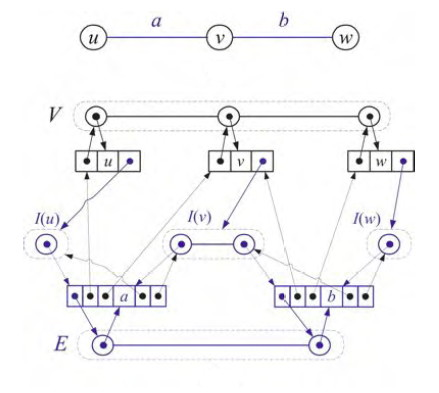
\includegraphics[width=0.5\textwidth]{1convderepr/schema.jpg}
         \caption{Liste d'adjacence}
          \label{adj}
\end{figure}

\subsection{Motivations}
Le fait de représenter un graphe avec la structure décrite précédemment possède divers avantages. Ceux-ci sont les suivants : \\

\begin{itemize}
\item \textbf{Facilité d'implémentation} : dans l'algorithme à implémenter, les actions principales à effectuer sur le graphe sont de trouver les arêtes sortantes d'un noeud, les noeuds vers lesquels elles se dirigent et de diminuer leur \textit{incounter}. L'implémentation de ces deux fonctionnalités est très facile car chaque objet contient les références nécessaires.

\item \textbf{Complexité satisfaisante} : la complexité temporelle de l'algorithme avec notre structure de données est en $\mathcal{O}(n + m)$ où $n$ et $m$ sont respectivement le nombre de noeuds et d'arêtes du graphe. Nous ne pourrions pas faire mieux étant donné qu'il va au pire effectivement falloir passer par tous les noeuds et les arêtes. Deux autres représentations de graphe existent : la \textit{edge list structure} et la \textit{adjacency matrix structure}. La première a une complexité en $\mathcal{O}(m)$ pour trouver les arêtes incidentes à un sommet alors qu'avec notre structure la complexité est en $\mathcal{O}(1)$. La matrice d'adjacence présente aussi des désavantages à ce niveau-là car trouver les arêtes incidentes à un noeud $v$ est en $\mathcal{O}(n)$.
\end{itemize}
\begin{frame}[allowframebreaks]{Théorie du problème}

Un \textbf{graphe dirigé}, ou orienté, est un triplet $(V,E,\psi)$ où:
\begin{itemize}
\item $V$ est un ensemble dont les éléments sont appelés sommets ou nœuds;
\item $E$ est un ensemble dont les éléments sont appelés arêtes;
\item $\psi$ est une fonction, dite fonction d'incidence, qui associe à chaque arête un couple de sommets. Ici, l'ordre au sein du couple de sommets a de l'importance, il signifie qu'un sommet est le nœud de départ de l'arête, l'autre étant le nœud d'arrivée.\\
\end{itemize}

%Un \textbf{parcours} est une suite $v_0e_1v_1e_2...e_nv_n$, où $v_1;v_2;...$ sont des sommets, et $e_1;e_2;...$ sont des arêtes. La longueur du parcours est son nombre d'arêtes $n$. Le sommet d'origine est $v_0$, le sommet de destination $v_n$. Les autres sommets sont dits intérieurs. Un parcours est fermé si $v_0 = v_n$.\\

%Un \textbf{chemin} est un parcours dont les sommets sont tous distincts.\\

\hspace{0.5cm}

Un \textbf{cycle} est un parcours fermé dont les sommets d'origine et intérieurs sont tous distincts. Un graphe qui ne contient pas de cycle est dit acyclique.

\end{frame}

\begin{frame}[allowframebreaks]{L'algorithme est juste}

Soit $G$ un graphe possédant n nœuds $v$ et $m$ arêtes $e$. Procédons par l'absurde, et supposons que tous les nœuds de $G$ possèdent une arête entrante, et que $G$ est acyclique.\\

\begin{itemize}
\item On choisit arbitrairement le nœud $v_i$, par hypothèse le nœud $v_i$ possède au moins une arête entrante. 
\item On choisit arbitrairement l'une des ces arêtes entrantes et on supprime les éventuelles autres arêtes entrantes de $v_i$, on arrive alors au nœud $v_j$, qui possède également au moins une arête entrante(par hypothèse).
\begin{itemize}
\item Soit on arrive à un nœud déjà visité et la démonstration est finie.
\item Soit on arrive à un nœud qu'on n'avait pas encore visité et on réitère l'algorithme.
\end{itemize}
\item Comme le nombre de nœuds de $G$ est fini, on arrive au dernier nœud (puisqu'on n'a pas de cycle jusqu'à présent). Hors, par hypothèse ce dernier nœud possède également une arête entrante qui ne peut pointer vers un autre nœud qu'un de ceux visité $\Rightarrow$ il y a un cycle et contradiction.
\end{itemize}

\end{frame}


\begin{frame}[allowframebreaks]{L'algorithme se termine}

Le graphe $G$ possède un nombre fini de nœuds et d'arêtes.\\

A chaque itération 
\begin{itemize}
\item Il ne reste aucun nœud $\Rightarrow$ Le programme s'arrête.
\item Tous les nœuds ont au moins une arête entrante $\Rightarrow$ Le programme s'arrête.
\item Il existe un nœud ne possédant pas d'arête entrante. Ce nœud (et ses arêtes) est retiré par l'algorithme. Comme le graphe $G$ possède, par hypothèse, un nombre fini de nœuds, il finit par se retrouver dans l'une des situations précédentes $\Rightarrow$ Le programme s'arrête.
\end{itemize} 

\end{frame}
\subsection*{Démonstration : L'algorithme est correct.}
\paragraph{\textit{Hypothèses :}}Soit $G$ un graphe possédant $n$ nœuds $v_i$ avec $i=1,...,n$ et $m$ arêtes $e_j$ avec $j=1,...,m$. Procédons par l'absurde, et supposons que $G$ possède un sous-graphe $H$ dont tous les noeuds possèdent une arête entrante, et que $G$ est acyclique.\\
\begin{itemize}
\item On choisit arbitrairement le nœud $v_i$ appartenant à $H$. Par hypothèse le nœud $v_i$ possède au moins une arête entrante. 
\item On choisit arbitrairement l'une des ces arêtes entrantes et on prend le noeud $v_j$ qui est l'origine de cette arête et qui possède également au moins une arête entrante (par hypothèse).
\begin{itemize}
\item Soit on arrive à un nœud déjà visité et la démonstration est finie.
\item Soit on arrive à un nœud qu'on n'avait pas encore visité et on réitère le point précédent.
\end{itemize}
\item Si tous les noeuds de $H$ ont été parcourus, comme le nombre de nœuds de $H$ est fini, on arrive au dernier nœud. Hors, par hypothèse ce dernier nœud possède également une arête entrante qui ne peut pointer vers un autre nœud qu'un de ceux visité $\Rightarrow$ il y a un cycle et donc il y a contradiction avec l'hypothèse de départ.
\end{itemize}
\subsection*{Démonstration : L'algorithme se finit toujours.}
\paragraph{\textit{Hypothèse :}}Le graphe $G$ possède un nombre fini de nœuds et d'arêtes.\\
A chaque itération, on observe plusieurs cas possibles : 
\begin{itemize}
\item Il ne reste aucun nœud $\Rightarrow$ Le programme s'arrête.
\item Tous les nœuds ont au moins une arête entrante $\Rightarrow$ Le programme s'arrête.
\item Il existe un nœud ne possédant pas d'arête entrante. Ce nœud (et ses arêtes) est retiré par l'algorithme. Comme le graphe $G$ possède, par hypothèse, un nombre fini de nœuds, il finit par se retrouver dans l'une des situations précédentes $\Rightarrow$ Le programme s'arrête.
\end{itemize} 

\end{document}

